
%% bare_conf.tex
%% V1.4b
%% 2015/08/26
%% by Michael Shell
%% See:
%% http://www.michaelshell.org/
%% for current contact information.
%%
%% This is a skeleton file demonstrating the use of IEEEtran.cls
%% (requires IEEEtran.cls version 1.8b or later) with an IEEE
%% conference paper.
%%
%% Support sites:
%% http://www.michaelshell.org/tex/ieeetran/
%% http://www.ctan.org/pkg/ieeetran
%% and
%% http://www.ieee.org/

%%*************************************************************************
%% Legal Notice:
%% This code is offered as-is without any warranty either expressed or
%% implied; without even the implied warranty of MERCHANTABILITY or
%% FITNESS FOR A PARTICULAR PURPOSE! 
%% User assumes all risk.
%% In no event shall the IEEE or any contributor to this code be liable for
%% any damages or losses, including, but not limited to, incidental,
%% consequential, or any other damages, resulting from the use or misuse
%% of any information contained here.
%%
%% All comments are the opinions of their respective authors and are not
%% necessarily endorsed by the IEEE.
%%
%% This work is distributed under the LaTeX Project Public License (LPPL)
%% ( http://www.latex-project.org/ ) version 1.3, and may be freely used,
%% distributed and modified. A copy of the LPPL, version 1.3, is included
%% in the base LaTeX documentation of all distributions of LaTeX released
%% 2003/12/01 or later.
%% Retain all contribution notices and credits.
%% ** Modified files should be clearly indicated as such, including  **
%% ** renaming them and changing author support contact information. **
%%*************************************************************************


% *** Authors should verify (and, if needed, correct) their LaTeX system  ***
% *** with the testflow diagnostic prior to trusting their LaTeX platform ***
% *** with production work. The IEEE's font choices and paper sizes can   ***
% *** trigger bugs that do not appear when using other class files.       ***                          ***
% The testflow support page is at:
% http://www.michaelshell.org/tex/testflow/



\documentclass[conference]{IEEEtran}
% Some Computer Society conferences also require the compsoc mode option,
% but others use the standard conference format.
%
% If IEEEtran.cls has not been installed into the LaTeX system files,
% manually specify the path to it like:
% \documentclass[conference]{../sty/IEEEtran}





% Some very useful LaTeX packages include:
% (uncomment the ones you want to load)


% *** MISC UTILITY PACKAGES ***
%
%\usepackage{ifpdf}
% Heiko Oberdiek's ifpdf.sty is very useful if you need conditional
% compilation based on whether the output is pdf or dvi.
% usage:
% \ifpdf
%   % pdf code
% \else
%   % dvi code
% \fi
% The latest version of ifpdf.sty can be obtained from:
% http://www.ctan.org/pkg/ifpdf
% Also, note that IEEEtran.cls V1.7 and later provides a builtin
% \ifCLASSINFOpdf conditional that works the same way.
% When switching from latex to pdflatex and vice-versa, the compiler may
% have to be run twice to clear warning/error messages.






% *** CITATION PACKAGES ***
%
%\usepackage{cite}
% cite.sty was written by Donald Arseneau
% V1.6 and later of IEEEtran pre-defines the format of the cite.sty package
% \cite{} output to follow that of the IEEE. Loading the cite package will
% result in citation numbers being automatically sorted and properly
% "compressed/ranged". e.g., [1], [9], [2], [7], [5], [6] without using
% cite.sty will become [1], [2], [5]--[7], [9] using cite.sty. cite.sty's
% \cite will automatically add leading space, if needed. Use cite.sty's
% noadjust option (cite.sty V3.8 and later) if you want to turn this off
% such as if a citation ever needs to be enclosed in parenthesis.
% cite.sty is already installed on most LaTeX systems. Be sure and use
% version 5.0 (2009-03-20) and later if using hyperref.sty.
% The latest version can be obtained at:
% http://www.ctan.org/pkg/cite
% The documentation is contained in the cite.sty file itself.






% *** GRAPHICS RELATED PACKAGES ***
%
\ifCLASSINFOpdf
  % \usepackage[pdftex]{graphicx}
  % declare the path(s) where your graphic files are
  % \graphicspath{{../pdf/}{../jpeg/}}
  % and their extensions so you won't have to specify these with
  % every instance of \includegraphics
  % \DeclareGraphicsExtensions{.pdf,.jpeg,.png}
\else
  % or other class option (dvipsone, dvipdf, if not using dvips). graphicx
  % will default to the driver specified in the system graphics.cfg if no
  % driver is specified.
  % \usepackage[dvips]{graphicx}
  % declare the path(s) where your graphic files are
  % \graphicspath{{../eps/}}
  % and their extensions so you won't have to specify these with
  % every instance of \includegraphics
  % \DeclareGraphicsExtensions{.eps}
\fi
% graphicx was written by David Carlisle and Sebastian Rahtz. It is
% required if you want graphics, photos, etc. graphicx.sty is already
% installed on most LaTeX systems. The latest version and documentation
% can be obtained at: 
% http://www.ctan.org/pkg/graphicx
% Another good source of documentation is "Using Imported Graphics in
% LaTeX2e" by Keith Reckdahl which can be found at:
% http://www.ctan.org/pkg/epslatex
%
% latex, and pdflatex in dvi mode, support graphics in encapsulated
% postscript (.eps) format. pdflatex in pdf mode supports graphics
% in .pdf, .jpeg, .png and .mps (metapost) formats. Users should ensure
% that all non-photo figures use a vector format (.eps, .pdf, .mps) and
% not a bitmapped formats (.jpeg, .png). The IEEE frowns on bitmapped formats
% which can result in "jaggedy"/blurry rendering of lines and letters as
% well as large increases in file sizes.
%
% You can find documentation about the pdfTeX application at:
% http://www.tug.org/applications/pdftex





% *** MATH PACKAGES ***
%
%\usepackage{amsmath}
% A popular package from the American Mathematical Society that provides
% many useful and powerful commands for dealing with mathematics.
%
% Note that the amsmath package sets \interdisplaylinepenalty to 10000
% thus preventing page breaks from occurring within multiline equations. Use:
%\interdisplaylinepenalty=2500
% after loading amsmath to restore such page breaks as IEEEtran.cls normally
% does. amsmath.sty is already installed on most LaTeX systems. The latest
% version and documentation can be obtained at:
% http://www.ctan.org/pkg/amsmath





% *** SPECIALIZED LIST PACKAGES ***
%
%\usepackage{algorithmic}
% algorithmic.sty was written by Peter Williams and Rogerio Brito.
% This package provides an algorithmic environment fo describing algorithms.
% You can use the algorithmic environment in-text or within a figure
% environment to provide for a floating algorithm. Do NOT use the algorithm
% floating environment provided by algorithm.sty (by the same authors) or
% algorithm2e.sty (by Christophe Fiorio) as the IEEE does not use dedicated
% algorithm float types and packages that provide these will not provide
% correct IEEE style captions. The latest version and documentation of
% algorithmic.sty can be obtained at:
% http://www.ctan.org/pkg/algorithms
% Also of interest may be the (relatively newer and more customizable)
% algorithmicx.sty package by Szasz Janos:
% http://www.ctan.org/pkg/algorithmicx




% *** ALIGNMENT PACKAGES ***
%
%\usepackage{array}
% Frank Mittelbach's and David Carlisle's array.sty patches and improves
% the standard LaTeX2e array and tabular environments to provide better
% appearance and additional user controls. As the default LaTeX2e table
% generation code is lacking to the point of almost being broken with
% respect to the quality of the end results, all users are strongly
% advised to use an enhanced (at the very least that provided by array.sty)
% set of table tools. array.sty is already installed on most systems. The
% latest version and documentation can be obtained at:
% http://www.ctan.org/pkg/array


% IEEEtran contains the IEEEeqnarray family of commands that can be used to
% generate multiline equations as well as matrices, tables, etc., of high
% quality.




% *** SUBFIGURE PACKAGES ***
%\ifCLASSOPTIONcompsoc
%  \usepackage[caption=false,font=normalsize,labelfont=sf,textfont=sf]{subfig}
%\else
%  \usepackage[caption=false,font=footnotesize]{subfig}
%\fi
% subfig.sty, written by Steven Douglas Cochran, is the modern replacement
% for subfigure.sty, the latter of which is no longer maintained and is
% incompatible with some LaTeX packages including fixltx2e. However,
% subfig.sty requires and automatically loads Axel Sommerfeldt's caption.sty
% which will override IEEEtran.cls' handling of captions and this will result
% in non-IEEE style figure/table captions. To prevent this problem, be sure
% and invoke subfig.sty's "caption=false" package option (available since
% subfig.sty version 1.3, 2005/06/28) as this is will preserve IEEEtran.cls
% handling of captions.
% Note that the Computer Society format requires a larger sans serif font
% than the serif footnote size font used in traditional IEEE formatting
% and thus the need to invoke different subfig.sty package options depending
% on whether compsoc mode has been enabled.
%
% The latest version and documentation of subfig.sty can be obtained at:
% http://www.ctan.org/pkg/subfig




% *** FLOAT PACKAGES ***
%
%\usepackage{fixltx2e}
% fixltx2e, the successor to the earlier fix2col.sty, was written by
% Frank Mittelbach and David Carlisle. This package corrects a few problems
% in the LaTeX2e kernel, the most notable of which is that in current
% LaTeX2e releases, the ordering of single and double column floats is not
% guaranteed to be preserved. Thus, an unpatched LaTeX2e can allow a
% single column figure to be placed prior to an earlier double column
% figure.
% Be aware that LaTeX2e kernels dated 2015 and later have fixltx2e.sty's
% corrections already built into the system in which case a warning will
% be issued if an attempt is made to load fixltx2e.sty as it is no longer
% needed.
% The latest version and documentation can be found at:
% http://www.ctan.org/pkg/fixltx2e


%\usepackage{stfloats}
% stfloats.sty was written by Sigitas Tolusis. This package gives LaTeX2e
% the ability to do double column floats at the bottom of the page as well
% as the top. (e.g., "\begin{figure*}[!b]" is not normally possible in
% LaTeX2e). It also provides a command:
%\fnbelowfloat
% to enable the placement of footnotes below bottom floats (the standard
% LaTeX2e kernel puts them above bottom floats). This is an invasive package
% which rewrites many portions of the LaTeX2e float routines. It may not work
% with other packages that modify the LaTeX2e float routines. The latest
% version and documentation can be obtained at:
% http://www.ctan.org/pkg/stfloats
% Do not use the stfloats baselinefloat ability as the IEEE does not allow
% \baselineskip to stretch. Authors submitting work to the IEEE should note
% that the IEEE rarely uses double column equations and that authors should try
% to avoid such use. Do not be tempted to use the cuted.sty or midfloat.sty
% packages (also by Sigitas Tolusis) as the IEEE does not format its papers in
% such ways.
% Do not attempt to use stfloats with fixltx2e as they are incompatible.
% Instead, use Morten Hogholm'a dblfloatfix which combines the features
% of both fixltx2e and stfloats:
%
% \usepackage{dblfloatfix}
% The latest version can be found at:
% http://www.ctan.org/pkg/dblfloatfix




% *** PDF, URL AND HYPERLINK PACKAGES ***
%
%\usepackage{url}
% url.sty was written by Donald Arseneau. It provides better support for
% handling and breaking URLs. url.sty is already installed on most LaTeX
% systems. The latest version and documentation can be obtained at:
% http://www.ctan.org/pkg/url
% Basically, \url{my_url_here}.




% *** Do not adjust lengths that control margins, column widths, etc. ***
% *** Do not use packages that alter fonts (such as pslatex).         ***
% There should be no need to do such things with IEEEtran.cls V1.6 and later.
% (Unless specifically asked to do so by the journal or conference you plan
% to submit to, of course. )


% correct bad hyphenation here
\hyphenation{op-tical net-works semi-conduc-tor}

\usepackage{graphicx}
\usepackage{subcaption}
\usepackage{wrapfig}
\usepackage{float}
\graphicspath{{./ReportImages/}}


\begin{document}
%
% paper title
% Titles are generally capitalized except for words such as a, an, and, as,
% at, but, by, for, in, nor, of, on, or, the, to and up, which are usually
% not capitalized unless they are the first or last word of the title.
% Linebreaks \\ can be used within to get better formatting as desired.
% Do not put math or special symbols in the title.
\title{American Sign Language Alphabet Recognition Using Computer Vision and Machine Learning Techniques}


% author names and affiliations
% use a multiple column layout for up to three different
% affiliations
\author{\IEEEauthorblockN{William Ritchie}
\IEEEauthorblockA{School of Computer Science\\
San Diego State University}
\and
\IEEEauthorblockN{Kristi Werry}
\IEEEauthorblockA{School of Computer Science\\
San Diego State University}}

% conference papers do not typically use \thanks and this command
% is locked out in conference mode. If really needed, such as for
% the acknowledgment of grants, issue a \IEEEoverridecommandlockouts
% after \documentclass

% for over three affiliations, or if they all won't fit within the width
% of the page, use this alternative format:
% 
%\author{\IEEEauthorblockN{Michael Shell\IEEEauthorrefmark{1},
%Homer Simpson\IEEEauthorrefmark{2},
%James Kirk\IEEEauthorrefmark{3}, 
%Montgomery Scott\IEEEauthorrefmark{3} and
%Eldon Tyrell\IEEEauthorrefmark{4}}
%\IEEEauthorblockA{\IEEEauthorrefmark{1}School of Electrical and Computer Engineering\\
%Georgia Institute of Technology,
%Atlanta, Georgia 30332--0250\\ Email: see http://www.michaelshell.org/contact.html}
%\IEEEauthorblockA{\IEEEauthorrefmark{2}Twentieth Century Fox, Springfield, USA\\
%Email: homer@thesimpsons.com}
%\IEEEauthorblockA{\IEEEauthorrefmark{3}Starfleet Academy, San Francisco, California 96678-2391\\
%Telephone: (800) 555--1212, Fax: (888) 555--1212}
%\IEEEauthorblockA{\IEEEauthorrefmark{4}Tyrell Inc., 123 Replicant Street, Los Angeles, California 90210--4321}}




% use for special paper notices
%\IEEEspecialpapernotice{(Invited Paper)}




% make the title area
\maketitle

% As a general rule, do not put math, special symbols or citations
% in the abstract
\begin{abstract}
American Sign Language (ASL) exists as a method of communication using physical gestures and hand signs instead of the verbal alternatives. We seek to bridge the gap between ASL users and non-ASL users by applying computer vision and machine learning techniques to images of the ASL alphabet. We propose a comparison of three methods for ASL alphabet recognition: error-correcting output code (ECOC) using multiple binary support vector machines (SVM) with histogram of oriented gradient (HOG) feature descriptors, bag of features (BOF) learning model with speeded-up robust features (SURF), and a convolutional neural network (CNN). Using an available 87000 image dataset, we trained these models with various parameters to see which one achieved highest accuracy in correctly classifying the ASL signs. We hypothesized the CNN would be the most successful in this task, due to its current prominence in the field of the computer vision. The results of our experiments show that the optimized version of ECOC using multiple binary SVM’s with HOG feature descriptors achieved the highest accuracy of the three models with 99.4 percent on only 29000 training images.
\end{abstract}

% no keywords


% For peer review papers, you can put extra information on the cover
% page as needed:
% \ifCLASSOPTIONpeerreview
% \begin{center} \bfseries EDICS Category: 3-BBND \end{center}
% \fi
%
% For peerreview papers, this IEEEtran command inserts a page break and
% creates the second title. It will be ignored for other modes.
\IEEEpeerreviewmaketitle



\section{Introduction}
% no \IEEEPARstart
Sign language is a language that is fundamentally different from any other language. Most languages are spoken or written; however, sign language is a complex language that uses the movement of hands, facial expressions, and body postures to convey a message. Each sign language also has its own grammar and lexicon. With the recent advancements in computer vision and machine learning, computer recognition of sign language is now feasible. With that said, there still exist a few problems in translating sign languages using current computer vision techniques, such as the number of complex signs and subtle motions that differentiate words and phrases. There is also a problem of non-uniformity amongst sign language users, in other words different sign language users might sign the same word slightly differently than another user. Another problem is the context provided by facial expressions. Such context can change the meaning of what is being said, thus making the need for facial recognition along with hand sign recognition valuable. There also exists a problem where the majority of people in the world are non-sign language users which can make communication between someone who uses sign language and a non-sign language user challenging. In this paper, we will focus on the hand signs of the alphabet for the American Sign Language (ASL). Convolutional neural networks (CNN) and support vector machine (SVM) are two of the more popular and successful machine learning techniques used to recognize an image of a signed letter. We chose SVM as opposed to other machine learning methods, due to its notoriety as a strong model for both binary and multi classification of images and because of its general simplicity to implement. CNN was chosen over other deep learning neural networks because it is specifically suitable for images as input whereas others are not. A big difference between CNN and other neural networks is that subregions might overlap, hence the neurons of a CNN produce spatially-correlated outcomes, whereas in other types of neural networks, the neurons do not share any connections and produce independent outcomes. In addition, in a neural network with fully-connected neurons, the number of parameters (weights) can increase quickly as the size of the input increases. A convolutional neural network reduces the number of parameters with the reduced number of connections, shared weights, and downsampling. We propose a comparison between these two techniques in tandem with various image processing and feature extraction algorithms such as histogram of oriented gradients (HOG) and speeded up robust features (SURF), to provide a highest accuracy model for ASL alphabet detection. The goal is to use the most accurate model to bridge the language gap between ASL users and non-users to make communication easier.
\begin{figure}[b]
\centering
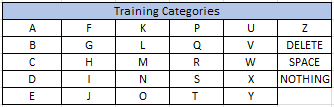
\includegraphics[width=\linewidth]{Categories_table1}
\caption{Training categories used for classifying ASL alphabet.}
\end{figure}
\section{Task Description}
We use image classification to assign category labels to images and test the correct classification. Figure 1 shows the 29 unique categories we used to classify the ASL alphabet [1]. The first 26 categories are the letters of the english alphabet, and the remaining three are: delete, space, and nothing. Delete and space are the sign language representation of those respective terms, and nothing represents no sign present (that is, no hand is present). 

\subsection{Error-Correcting Output Code with SVM Binary Learners}
The process of assigning categories involves collecting unique features over a collection of training images in a specific category, and applying a machine learning model to learn the collection of features in each category. The first method we propose involves an error-correcting output code (ECOC) multi-class model using SVM binary learners, to learn the features extracted by applying the HOG algorithm on the dataset. ECOC classification requires a coding design which determines the classes that the binary learners train on, and a decoding scheme, which determines how the results (predictions) of the binary classifiers are aggregated [2]. A coding design is a matrix where elements direct which classes are trained by each binary learner, that is, how the multiclass problem is reduced to a series of binary problems [2]. HOG is an algorithm that extracts a feature descriptor for object detection from images. It does this by counting each instance of gradient orientation at specific points of an image. The appearance and shape of an image can be described through the intensities and directions of the gradients. These features are useful because the gradient magnitudes are usually larger around corners and edges which can tell a lot about an object. Figure 2 shows the result of applying HOG on an image of a signed letter. As you can see the larger gradient magnitudes around the edges of the hand. 
\begin{figure}[h]
\centering
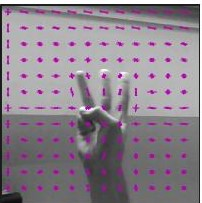
\includegraphics[width=0.5\linewidth]{HOG_W_sign}
\caption{HOG features of the ASL sign `W'.}
\end{figure}
The resulting features from applying HOG are used as an input to the ECOC model, which selects the most optimal features to provide classification of the image. Each SVM binary learner searches for an optimal hyperplane that separates the data into two classes. For separable classes the optimal hyperplane maximizes a margin surrounding itself (space that does not contain any observations), which creates boundaries for the positive and negative classes [3]. 

\subsection{Bag Of Features with Speeded Up Robust Features Descriptors}
After further investigation, we decided to compare HOG against SURF which is a fast approximation of scale-invariant feature transform (SIFT). The SIFT descriptor is based on HOG, so we expected the faster and more efficient SURF algorithm to yield higher results. In Figure 3 you can see the results of applying SURF on an image. 
\begin{figure}[h]
\centering
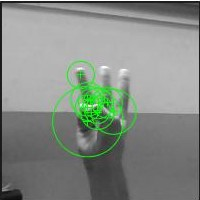
\includegraphics[width=0.5\linewidth]{SURF_W_sign}
\caption{SURF features of the ASL sign `W'.}
\end{figure}
We realized we could not use SURF with ECOC due the varying number of features per image, leading us to the second proposed method for ASL alphabet recognition, called bag of features (BOF). BOF still utilized SVM and naturally handled the issues presented by SURF. To detect interest points, SURF uses an integer approximation of the determinant of Hessian blob detector, which can be computed using a precomputed integral image. Its feature descriptor is based on the sum of the Haar wavelet response around the point of interest [5]. BOF constructs a “vocabulary” of SURF feature descriptors representative of each image category. In constructing this vocabulary it reduces the number of features through quantization of feature space using K-means clustering. Then, based on results of the clustering, it counts the visual word occurrences in each image and produces a histogram that becomes a new and reduced representation of each image. This histogram forms a feature vector of an image, which is then fed into a multiclass linear SVM classifier during the training process [4].
\subsection{Convolutional Neural Network}
The third method we propose for ASL alphabet recognition is training a CNN. A CNN eliminates the need for manual feature extraction as the features are learned directly by the CNN. Filters are applied to each training image at different resolutions, and the output of each convolved image is used as the input to the next layer. The filters become complex features that uniquely define the object. CNN is composed of an input layer, many hidden layers, and then an output layer. These layers perform operations that alter the data with the intent of learning features specific to the data. The three most common middle layers are: convolution, ReLU (activation), and pooling. Convolution puts the input images through a set of convolutional filters, each of which activates certain features from the images. Rectified linear unit (ReLU) allows for faster and more effective training by mapping negative values to zero and maintaining positive values. This is sometimes referred to as activation, because only the activated features are carried forward into the next layer. Pooling simplifies the output by performing nonlinear downsampling, reducing the number of parameters that the network needs to learn. Following these layers are the classification layers which is comprised of a fully connected layer that contains the probabilities for each class of any image being classified, and a softmax layer to provide the classification output. There are different types of CNN such as R-CNN, Fast R-CNN, and Faster R-CNN. While those models have been proven to be successful we decided to go with our own implementation of a CNN in order to have more control over the network and attempt to produce equally impressive results. \\

For each of the proposed methods we conducted experiments in an attempt to maximize the accuracy of each model. These experiments involved manipulating many of the parameters under which the different models could run and observing how those manipulations affected the accuracy. The set of parameters that provided the highest accuracy model was then compared against the other methods using the same exact set of training and testing images. 
\section{Major challenges and Solutions}
Our greatest challenge was lack of adequate resources to train the machine learning models. Normally these models would run on clusters of CPU’s or GPU’s to drastically decrease the time it takes to train the model. Despite the fact that our training images were small in size and in some cases we converted the entire image set to grayscale, training time still could take many hours to finish (the more extreme cases being upwards of 12 hours). During those hours of training, the huge number of extracted features completely filled the computer's memory and the bus lines to disk would be completely taken up, preventing us from doing much else while the models trained. We did not have the money to purchase multiple CPUs or highly expensive GPUs. Our solution was to use an alternate computer in order to continue to work while the other computer trained the models, thus optimizing our time. We also set the settings for the CNN to multi-CPU (parallel processing) to help speed up the process. We still ran into the issue where some of the models were so exhaustive that they crashed the computers which meant we had to restart the training of the model. There was no straightforward solution to this; instead we accounted for failed model training sessions in the estimated time it would take for us to train all of the models. Our lack of hardware and resources definitely slowed down our testing, but we were able to produce results after an abundant amount of time. 
\section{Experiments}
\subsection{Dataset description}
The data set we used to train and test our machine learning models was downloaded from kaggle.com\footnote{The ASL alphabet image dataset we used can be found at the website Kaggle.com and it provided us with a collection of 87,000 images. There are 29 classes, 26 for each letter (A-Z) and 3 for Space, Delete, and Nothing. Each class has 3,000 images and each image is 200 by 200 pixels.}. The training data set is split into 3000 images per category, with there being 29 different categories (26 for each ASL letter in the alphabet and 3 for delete, space, and nothing). The 29 categories are those previously mentioned in the first paragraph of Task Description, and are the same as the labels we used in our classifications for training the models. The maximum number of images we trained per category was 2800 due to the constraints previously mentioned in Major Challenges and Solutions. The images are close up pictures of the hand producing the sign, thus the signs took up most of the space in the image. Each image varies from a solid to a very noisy background. These images also range from dark pictures to brightly lit photos. These different types of images of the same object help us train our models and make them more robust. The dataset also includes images for testing, with one image to test per category. We decided to not use these 29 images and instead use 200 (per category) of the remaining images from the original 3000 (per category). We felt this would give a more accurate result from the testing process.
\subsection{Evaluation Metrics}
\subsubsection{Parameters}
The experiment consisted of manipulating the various parameters to our three proposed methods of ASL alphabet recognition in order to achieve the highest accuracy possible. Since the different methods are very different in design, their respective parameters do not correlate to the other models. This means each model has its own experiment of altering parameters, and the only comparison that occurs between the different models is with respect to the highest accuracy achieved for each model. Thus, it is necessary to also self-compare the models, and understand why certain parameter values for a particular model may have caused higher accuracy. 

Due to our lack of resources (previously mentioned in the Major Challenges and Solutions section) we only increased the number of training images for the parameters that yielded better results. The increase amount is as follows: 300 images (per category) for the parameters with better results from the 100 training images (per category) run, and 2800 images (per category) for the singular run that performed the best in the previous 300 image (per category) run. Occasionally we trained with 1000 images (per category) if we felt 2800 was too computationally intensive.

For the ECOC model we used two of Matlab’s built-in functions: ‘fitcecoc’ and ‘extractHOGFeatures’. The ‘extractHOGFeatures’ extracts HOG features from a particular grayscale image, and the result is stored into a matrix. This step repeats for each image in the training image data set. The resulting matrix is used as an input to ‘fitcecoc’, which takes those features and a vector with the actual labels for the respective images, to train the multiple binary SVMs.

The parameters that we felt were worth considering for extracting HOG features were: ‘InterestPoints’, ‘CellSize’, ‘BlockSize’, and ‘NumberOfBins’. We decided not to use interest points from a corner or edge detector as an input to the function. Our reasoning behind this is that our training image dataset consists of close up photos of the hand sign with little background noise, thus we felt no need to detect interest points and that applying HOG over the entire image was sufficient. This also makes the model more closely related to the CNN model, since the CNN also extracts features over the entire image. In our conclusion and future works we discuss more on using interest points as an input to the HOG algorithm and to CNN (forming essentially an R-CNN model). Block size refers to the number of cells in a block. A large block size value reduces the ability to suppress local illumination changes. Reducing block size helps to capture the significance of local pixels and help suppress illumination changes of HOG features [7]. The default block size was set to 2 x 2, which we felt was sufficiently small and increasing the size did not seem desirable so we decided to not have block size be a parameter that we would change. The number of bins refers to the number of orientation histogram bins. Increasing this value increases the size of the feature vector, which requires more time to process, but is able to encode finer orientation details. The default number of bins is 9, and we decided not to change this value because it seems to be the standard in literature [7]. Cell size refers to the size of the HOG cell, which is used to capture spatial information. Increasing the cell size captures large scale spatial information, but loses small-scale detail. We decided this was an important parameter worth altering for the experiment. The value of cell size is a 2 element vector. 

For the ‘fitcecoc’ function, there are two parameters we felt were worth considering: ‘Coding’ and ‘Learners’. ‘Coding’ refers to how a multiclass problem is turned into a series of binary classifiers. Among the different options for the coding parameter two stood out as the most probable for success: ‘onevsone’ and ‘onevsall’. One versus one is where for each binary learner, one class is positive, another is negative, and the rest are ignored. This design exhausts all combinations of class pair assignments. One versus all is where for each binary learner, one class is positive and the rest are negative. This design exhausts all combinations of positive class assignments [8]. The other parameter we considered was the ‘Learner’ which refers to the type of binary classifier. As previously stated, we desired the binary classifier to be SVM, which happened to be what ‘fitcecoc’ was set to use as a default. The default kernel for the templateSVM class Matlab provides, is a linear model. In our experimentation we tried both a gaussian kernel and the linear kernel [14].

We used the built-in Matlab functions ‘bagOfFeatures’ and ‘trainImageCategoryClassifier’ for the BOF model. The ‘bagOfFeatures’ function takes in our dataset as an input, and begins by extracting SURF features.This bagging step was helpful because SURF would return varying number of features per image, thus making it difficult to compare and learn using fitcecoc. All of the relevant features were placed in a ‘bagOfFeatures’ object which is used as an input to the ‘trainImageCategoryClassifier’ method. This trains an SVM using the dataset with the category labels along with the bag of features. 

A few important parameters for ‘bagOfFeatures’ are: ‘StrongestFeatures’, ‘PointSelection’, ‘GridStop’, and ‘BlockWidth’. ‘StrongestFeatures’ allows us to pick a percentage of the best features [9]. By default, this is 80 percent; however, this produced a large amount of features that took a huge amount of time to process. We changed this to 50 percent to speed up computation and after testing on a small scale we realized the accuracy was slightly less, and felt the increased computation time in this case was worth the increase in accuracy so we kept this parameter at 80 percent. ‘PointSelection’ has two options for the method of picking point locations. We decided with ‘Detector’ because it selects point based on SURF whereas ‘Grid’ picked points based on a predefined grid. Since we did not use ‘Grid’ in the point selection, there was no reason to change the ‘GridStep’ parameter. For ‘BlockWidth’, we also left this as default [32 64 96 128]. The minimum block width is 32, thus we could not make this smaller. On the other hand, since our images are only 200 by 200 pixels, and based on our previous experimenting with larger block widths, we decided we did not want to make the block widths any larger in fear of losing important features.

The only parameter that would change the accuracy of the training model ‘trainImageCategoryClassifier’ was the ‘LearnerOptions’ [10]. This function trains a multi-class SVM. Like the ‘fitcecoc’ function, we decided to use a Gaussian filter for training to help reduce noise. 

Creating a custom CNN was significantly different from training the other models. The CNN only has two requirements for its layers: to begin with an image input layer, and to end with an output (classification) layer. The layers in between can be anything. The large freedom in number of layers and types of layers makes creating a custom CNN very time consuming, and so for the scope of this project we tried to limit ourselves. After specifying the layers of the CNN, we also needed to specify the options under which the CNN would train. These options include: the ‘MaxEpochs’, ‘MiniBatchSize’, ‘InitialLearnRate’, along with many others. Both the layers, the options, and the image dataset with the image labels are then given to the function: ‘trainNetwork’, which will train the CNN. 

The first layer in every CNN is the image input layer which defines the image size; in this case, 200 by 200 by 3. We decided to use the RGB colors and not change the original images to grayscale because this would give the neural network more information to work with while traversing through the other layers. In Matlab this functionality is achieved with the ‘imageInputLayer’ function. This function has three parameters worth noting: ‘Normalization’, ‘AverageImage’, and ‘DataAugmentation’. The ‘Normalization’ parameter defaults to ‘zerocenter’, which subtracts the average image specified by the average image property. We felt this normalization technique was sufficient and did not need to be changed. Likewise the ‘AverageImage’ property defaulted to a h-by-w-by-c array, which was designed for the ‘Normalization’ parameter which we decided to change. The ‘DataAugmentation’ parameter would have been useful except we already augmented the training data prior to this layer, therefore we kept this value as ‘none’. The reasoning behind our data augmentation is discussed later in this section. The next layer is usually a convolutional layer which applies a number of filters of a specific size on the padded images. The goal of the convolutional layer is to activate the key interest points of the image. We achieved this by using Matlab’s ‘convolution2dLayer’. This function has many possible input parameters, so for the scope of this project we limited ourselves to these few: ‘FilterSize’, ‘NumFilters’, ‘PaddingMode’, and ‘PaddingSize’. There are other important parameters to this function that we chose not to try such as: ‘Weights’ and ‘Bias’. We felt the ‘Weights’ and ‘Bias’ was out of scope and left those parameters to their default values. The batch normalization layer usually follows the convolutional layer. This layer normalizes the activations and gradients from the convolution layer to optimize the network training. Following the batch normalization layer, the ReLU layer is the most common to use for nonlinear activation. Both the batch normalization layer and the ReLU layer seemed to be the standard and the corresponding Matlab functions did not take in many inputs so we decided to leave these layers at their default settings. At this point there is usually a very large feature map. We used a down-sampling layer like max pooling layer to remove the redundant spatial information. Down-sampling makes it possible to increase the number of filters in deeper convolutional layers without increasing the required amount of computation per layers. This functionality was achieved using Matlab’s built-in function: ‘maxPooling2dLayer’. The primary parameters we modified for this function were: ‘PoolSize’ and ‘Stride’. The pool size refers to the dimensions of the pooling regions. The stride is the step size for traversing the input vertically and horizontally. After the first pooling layer, we attempted repeating and trying different combinations of the convolutional layer, batch normalization layer, ReLU, and max pooling layer. Regardless of the different combinations, the last three layers were always the same. The first is the fully connected layer. The fully connected layer connects to all of the features from previous layers across the image to identify a pattern which is used to classify the image. We used Matlab’s ‘fullyConnectedLayer’ function to achieve the necessary functionality of this layer. This function has an input of output size, this number corresponds to the number of different classifications. There was no need to experiment with the input to this function since it was set to the number of classes we had, thus 29 was the input. Other possible parameters included ‘Weights’ and ‘Bias’, which (as we previously have mentioned) are out of the scope of this assignment and left those parameters at their default values. Following the fully connected layer is the soft max layer. The soft max layer normalizes the fully connected layer and creates a single positive number used for classification probability. We used Matlab’s: ‘softmaxLayer’ function. This function did not take in any relevant inputs. The last layer is the classification layer. The classification layer uses the probability from the soft max layer to assign input into one of the mutually exclusive class and computes the loss. Matlab’s ‘classificationLayer’ function also does not have any relevant input parameters. 

After an initial run with basic layer and option parameters, we got decent cross-validation results around 85 percent, but our validation results with the test images were very poor (approximately 35 percent). Therefore, we decided to add an image data augmenter to preprocess the training images. This would change the images in the dataset by rotating and translating randomly. This would help the CNN be more robust against images not in our dataset. This change to pre-processing significantly increased the accuracy of our CNN. 

The primary options for the CNN we explored were: ‘InitialLearnRate’, ‘LearnRateDropPeriod’, ‘MaxEpochs’, ‘MiniBatchSize’, ‘LearnRateSchedule’, ‘L2Regularization’, ‘Shuffle’, and the ‘ExecutionEnvironment’. We felt that these were the major options that would affect the training accuracy. The default ‘MaxEpochs’ is 30, but we found that 20 full passes of the training algorithm over the entire training set was sufficient enough for the model to learn from our data. The ‘MiniBatchSize’ is the size of the training subset used to evaluate the gradient loss and update the weights of our model. After testing different sizes, we found that 64 was the most optimal for our dataset because it provided more updated information than the default 128 mini batch size. We set the ‘Shuffle’ parameter to ‘every-epoch’ because we did not want the model to learn the order in which the images appear. We played around with ‘InitialLearnRate’ because if the learning rate is too low then training takes a long time, but if the rate is too high then training might reach a suboptimal result or diverge. We also wanted to know how changing the ‘LearnRateSchedule’ would affect the training process. By default, the learning rate was constant, but theorized it might be beneficial to change the rate to decrease in piecewise manner in order to save time and increase accuracy. We determined the results from changing the learning rate were not as beneficial as we had hoped, so we kept this parameter at constant. We could also define a specific epoch that the learn rate would change at with learn rate drop period. ‘L2Regularization’ changed the amount of weight decay. The last option was changed almost immediately was the ‘ExecutionEnvironment’. By default, CNN training runs on a single CPU, which would not take the computer’s entire resources; however, this took a tremendous amount of time. Thus, we switched to parallel computing on multiple CPUs.
\subsubsection{Accuracy}
Accuracy is the primary metric we looked at in determining the best parameters for each model, as well as determining the overall best model for ASL alphabet recognition. In this case, accuracy refers to a trained model’s ability to correctly classify an image of an ASL sign with in the test set of images. Our project did not use the data set’s test images; instead, we used the remainder of the unused training images as the test set. We felt this provided a more robust accuracy result. Calculating the accuracy for the CNN required use of Matlabs ‘classify’ function, which gets the label predictions for all of the images in the testing set, compares them to the correct corresponding labels, sums together the number of correctly classified images and divides by the total number of testing images. In calculating the accuracy for the ECOC and BOF models, we used the sum of the diagonal of the confusion matrices and divided by the number of the test images. The confusion matrix used the result of Matlab’s built-in ‘predict’ function.
\begin{figure*}[t]
\centering
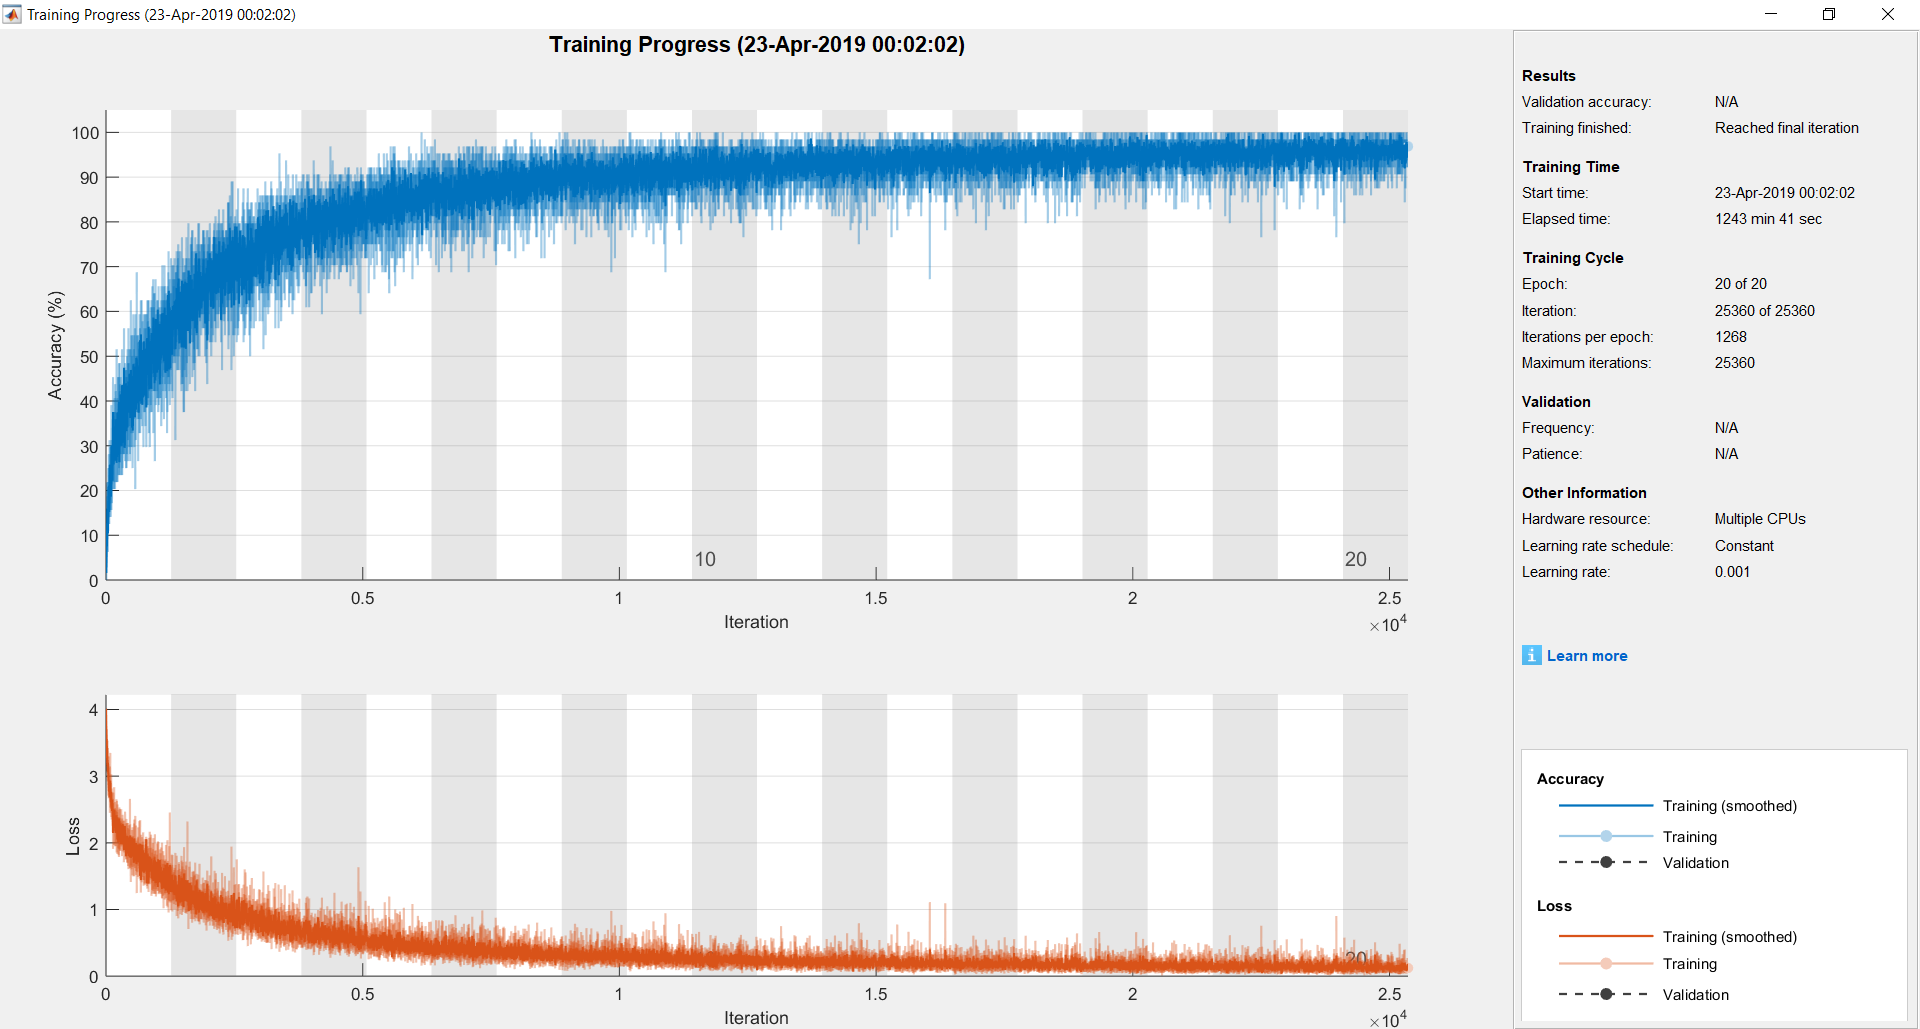
\includegraphics[width=\linewidth]{FinalTraining}
\caption{Training plot for the CNN.}
\end{figure*}
\subsubsection{Loss}
Although we did not use loss in determining the best model, we did take it into consideration. We only looked at the loss of the CNN because it was only relevant to this model. Over time we expected loss to decrease in value, producing a graph similar to that of exponential decay. Unlike accuracy, loss is a summation of errors and not a percentage. Reducing the loss value depends on changing the CNN’s weight vector values through different optimization techniques. A plot of our most accurate CNN model’s loss after the training phase can be seen in Figure 4. We took loss into consideration while creating, training, and testing our custom CNN to attain the best accuracy with a minimal loss during the training phase.

\subsubsection{Confusion Matrix}
We used confusion matrices for both of the SVMs to see an overview of the performance of the classification algorithm with respect to the different categories. Calculating a confusion matrix can show where the classification model is succeeding, but more importantly, what kind of errors the model is making. We used these matrices to optimize our accuracies in the SVM methods while testing different training options. We used loss to improve optimization for the CNN, thus had no need for a confusion matrix. Matlab provides a function that creates the confusion matrix called: ‘confusionmat’ which takes in an input of the predicted test image labels (determined using the ‘predict’ function) and the correct corresponding labels.
\subsection{Major Results}
Each classification model went through vigorous experimenting to find the best accuracy for the model. Each model would then be compared to the accuracy of the other models to find the overall best performing accuracy of ASL alphabet recognition.
\subsubsection{Error-Correcting Output Code with SVM Binary Learners}
After testing the different cell sizes, we found that using a 32 by 32 cell produced the best accuracy. Once we increased our number of training images per category from 100 to 300, we saw a significant increase in accuracy when using a Gaussian filter combined with the one vs all method. As you can see in Figure 5, run 11 shows this with a 95 percent accuracy. At this point, we decided to increase the number of training images per category to 1000 with a 32 by 32 cell size, Gaussian filter, and ‘onevsall’ method. We tested the 200 images per category (the same set tested on the other models) on this trained SVM model which produced a 99.4 percent accuracy.
\begin{figure}[b]
\centering
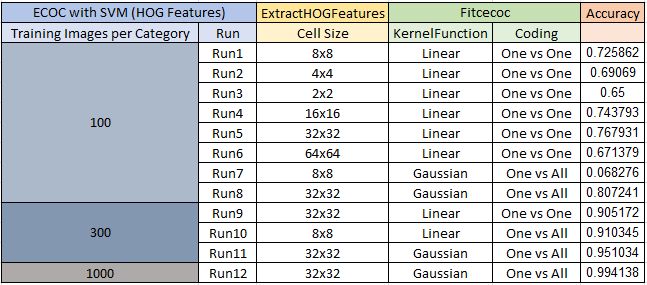
\includegraphics[width=\linewidth]{ECOC}
\caption{Accuracy results for the ECOC.}
\end{figure}

\subsubsection{Bag Of Features with Speeded Up Robust Features Descriptors}
Our initial runs tested whether using a ‘Grid’ or a ‘Detector’ to find SURF features generated better accuracy. Using the ‘Detector’ gave better accuracy for our small training set. Then we tested if using a Gaussian filter would perform any better, which it did. The results from this test can be seen in Figure 6. From there, we increased our training set to first 1000 images per category then finally to 2800 training images per category while using a ‘Detector’ and a Gaussian filter. Testing using the remaining 200 images per category finished with a 98.6 percent accuracy.
\begin{figure}[h]
\centering
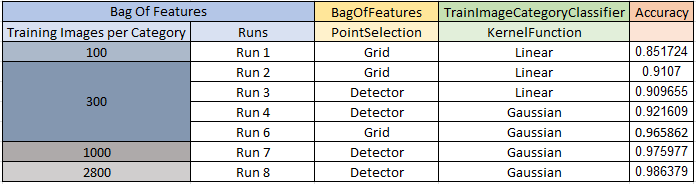
\includegraphics[width=\linewidth]{SURFSVM}
\caption{Accuracy results for the BOF.}
\end{figure}

\subsubsection{Convolutional Neural Network}
After experimenting with the different layers of the CNN, we decided to go with the following (in chronological order): image input layer, convolutional layer with 4 filters with a size of 4x4 and zero padding, a batch normalization layer, a ReLU layer, a max pooling layer with a stride of 2, followed by another convolutional layer with 8 filters each with a size of 4x4 and zero padding, another batch normalization layer, a ReLU layer, followed by another max pooling layer with the same inputs as the previous one, then the final convolutional layer with 16 filters with a size 4x4 and zero padding, a batch normalization layer, ReLU layer, then the fully connected layer, the softmax layer, and finally the classification layer. This exact sequence of layers and inputs yielded the best accuracy for CNN. You can see the results of our experimenting with different layers and parameters in Figure 8. Along with these layers, we decided our options would be: sgdm, 20 max epochs, 0.001 initial learn rate, 64 mini batch size, and default for learn rate schedule, learn rate drop period, and L2 regularization. We trained 2800 images per category and tested the remaining 200 which produced a 98.7 percent accuracy.

\subsubsection{Machine Model Comparison}
We took the best performing from each model and compared the accurracies. As you can see in Figure 7, extracting HOG features with an error correcting SVM did the best with a 99.4 percent accuracy.
\begin{figure}[h]
\centering
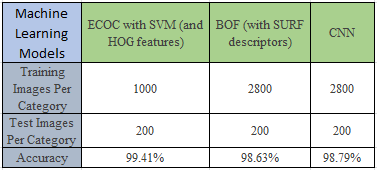
\includegraphics[width=\linewidth]{Overview}
\caption{Accuracy results for the machine learning models.}
\end{figure}
\begin{figure*}[h]
\centering
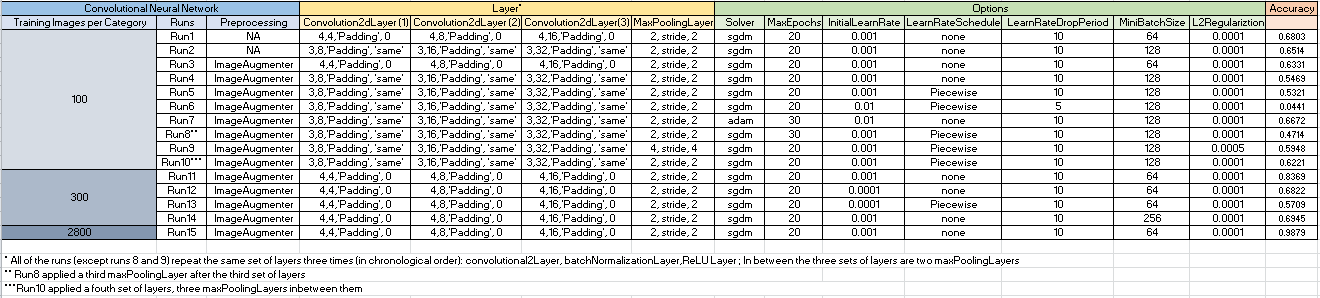
\includegraphics[width=\linewidth]{CNN}
\caption{Accuracy results for the CNN.}
\end{figure*}
\subsection{Analysis}
\subsubsection{Error-Correcting Output Code with SVM Binary Learners}
The range of cell size values we experimented with were: 2x2, 4x4, 8x8, 16x16, 32x32, and 64x64. Interestingly, 32 by 32 cell size yielded the best results with a 76.8 percent accuracy with 100 training images per category. We suspect the success of this large cell size is due to each training image being a close up of the hand sign and thus the large spatial information consisted primarily of the object of interest. 64x64 was likely too large in comparison to the 200x200 images and likely lost information about the hand sign. We suspected SVM learners that also applied a Gaussian filter improved accuracy due the smoothing effect that reduced noise. We expected ‘onevsall’ would outperform ‘onevsone’ since it seemed to more closely address our specific use case, were if one hand sign is recognized then it cannot be any of the other hand signs so assign them to a negative class as opposed to ignoring them. 
\subsubsection{Bag Of Features with Speeded Up Robust Features Descriptors}
Applying the Gaussian filter likely increased the accuracy due to filtering out noise. The point selection method from ‘Grid’ to ‘Detector’ is something we are inconclusive about. While the interest points provided by ‘Grid’ yielded better results, the huge number of points filled up the entirety of our memory for any run beyond 300 training images per category. Because of this inefficiency with use of space and our lack of a sufficient amount of memory we decided the ‘Detector’ was the most accurate, but we suspect if there was sufficient memory then ‘Grid’ would outperform ‘Detector’ at 2800 training images per category.
\subsubsection{Convolutional Neural Network}
Augmenting the training data set in terms of rotation and translation distinctly made the model more robust. This is likely because the network could end up just memorizing the training set and any slight deviation could be wrongly classified (this is shown by our results from a test we previously mentioned). As to why the number of filters from 4 to 8 to 16 did better than 8 to 16 to 32, is something we are not sure on. Originally we expected the larger number of filters (which directly corresponds to the number of neurons at that layer) to yield higher accuracy. We felt that more neurons meant more knowledge from the images was being extracted. We suspect now it might have more to do with essential information being spread out too far across the neurons and basically get lost by the time the fully connected layer is reached.The larger filter size, 4x4 compared to 3x3, is something we correctly hypothesized would yield better results. We hypothesized the smaller filter would not able to gather appropriate information about the images since they were zoomed in to the hand sign. This reasoning has a similar basis to our reasoning behind the cell size parameter in ECOC. The ‘MiniBatchSize’ was found to be most successful at 64, since this is the number of images used by stochastic gradient descent to update the parameters of the CNN, we were surprised to see a smaller mini batch size yield the best results, we expected that a larger number images to update the parameters with would provide a better and more accurate result.
\subsubsection{Overall}
It is interesting that the ECOC with SVM binary learners and HOG features did better than the CNN, since this model only used 1000 training images per category to yield the highest results. Whereas both of the other models had more images to train from (2800 per category). We expected the CNN to outperform the other models due to its popularity and success in the field of computer vision. This is likely because our knowledge of CNN and BOF is limited, whereas we knew more about HOG features and SVM allowing us to better fine tune the parameters. It would have been interesting to see if ECOC would have remained the most accurate model if we had been able to completely train the BOF model with a ‘Grid’ point selection method. Also, due to our limited resources (mentioned in Major Challenges and Solutions) and limited time, it was not within the scope of this project to test every parameter, and likely some of the parameters we chose to not adjust for the other models would have likely increased the accuracy. 
\section{Conclusion and Future Works}
Sign language is a visual language that uses hand signs, facial expressions, and body postures to convey information. We used computer vision and machine learning to create a model for sign language recognition. Our original goal was to produce an accurate classification model to eliminate the language gap between ASL users and non-users to ease communication. Each of our proposed models performs exceptionally well to identify the ASL alphabet. The best accuracy of all the models is using error-correcting output code using multiple binary support vector machines trained on histogram of oriented gradient features which produced a 99.4 percent accuracy. However, our model only recognizes the letters in the alphabet for ASL. It is possible to spell out every word using the alphabet, but this would not be very helpful in the real world where hand signs usually use represent words or phrases. Thus, to improve on our model, it would be practical to be able to recognize many different words in the language and not just the alphabet. Also, sign language users may sign words differently than others; the model must be made more robust in order to still be able to accurately recognize these words. It is also possible to sign without using any facial expressions or body movements, but doing so might be confusing or cause misunderstandings. Therefore, creating a facial expression, body posture model, as well would be beneficial in recognizing the entire message in ASL. We propose detecting interest points to find the regions of interest and using that information as inputs to our CNN and ECOC models. For CNN there is a specific version called region convolutional neural network (R-CNN) that achieves exactly that. The ability to accurately recognize hand signs, facial expressions, and body postures will close the language gap between ASL users and non-users to make communication easier.


% An example of a floating figure using the graphicx package.
% Note that \label must occur AFTER (or within) \caption.
% For figures, \caption should occur after the \includegraphics.
% Note that IEEEtran v1.7 and later has special internal code that
% is designed to preserve the operation of \label within \caption
% even when the captionsoff option is in effect. However, because
% of issues like this, it may be the safest practice to put all your
% \label just after \caption rather than within \caption{}.
%
% Reminder: the "draftcls" or "draftclsnofoot", not "draft", class
% option should be used if it is desired that the figures are to be
% displayed while in draft mode.
%
%\begin{figure}[!t]
%\centering
%\includegraphics[width=2.5in]{myfigure}
% where an .eps filename suffix will be assumed under latex, 
% and a .pdf suffix will be assumed for pdflatex; or what has been declared
% via \DeclareGraphicsExtensions.
%\caption{Simulation results for the network.}
%\label{fig_sim}
%\end{figure}

% Note that the IEEE typically puts floats only at the top, even when this
% results in a large percentage of a column being occupied by floats.


% An example of a double column floating figure using two subfigures.
% (The subfig.sty package must be loaded for this to work.)
% The subfigure \label commands are set within each subfloat command,
% and the \label for the overall figure must come after \caption.
% \hfil is used as a separator to get equal spacing.
% Watch out that the combined width of all the subfigures on a 
% line do not exceed the text width or a line break will occur.
%
%\begin{figure*}[!t]
%\centering
%\subfloat[Case I]{\includegraphics[width=2.5in]{box}%
%\label{fig_first_case}}
%\hfil
%\subfloat[Case II]{\includegraphics[width=2.5in]{box}%
%\label{fig_second_case}}
%\caption{Simulation results for the network.}
%\label{fig_sim}
%\end{figure*}
%
% Note that often IEEE papers with subfigures do not employ subfigure
% captions (using the optional argument to \subfloat[]), but instead will
% reference/describe all of them (a), (b), etc., within the main caption.
% Be aware that for subfig.sty to generate the (a), (b), etc., subfigure
% labels, the optional argument to \subfloat must be present. If a
% subcaption is not desired, just leave its contents blank,
% e.g., \subfloat[].


% An example of a floating table. Note that, for IEEE style tables, the
% \caption command should come BEFORE the table and, given that table
% captions serve much like titles, are usually capitalized except for words
% such as a, an, and, as, at, but, by, for, in, nor, of, on, or, the, to
% and up, which are usually not capitalized unless they are the first or
% last word of the caption. Table text will default to \footnotesize as
% the IEEE normally uses this smaller font for tables.
% The \label must come after \caption as always.
%
%\begin{table}[!t]
%% increase table row spacing, adjust to taste
%\renewcommand{\arraystretch}{1.3}
% if using array.sty, it might be a good idea to tweak the value of
% \extrarowheight as needed to properly center the text within the cells
%\caption{An Example of a Table}
%\label{table_example}
%\centering
%% Some packages, such as MDW tools, offer better commands for making tables
%% than the plain LaTeX2e tabular which is used here.
%\begin{tabular}{|c||c|}
%\hline
%One & Two\\
%\hline
%Three & Four\\
%\hline
%\end{tabular}
%\end{table}


% Note that the IEEE does not put floats in the very first column
% - or typically anywhere on the first page for that matter. Also,
% in-text middle ("here") positioning is typically not used, but it
% is allowed and encouraged for Computer Society conferences (but
% not Computer Society journals). Most IEEE journals/conferences use
% top floats exclusively. 
% Note that, LaTeX2e, unlike IEEE journals/conferences, places
% footnotes above bottom floats. This can be corrected via the
% \fnbelowfloat command of the stfloats package.

% trigger a \newpage just before the given reference
% number - used to balance the columns on the last page
% adjust value as needed - may need to be readjusted if
% the document is modified later
%\IEEEtriggeratref{8}
% The "triggered" command can be changed if desired:
%\IEEEtriggercmd{\enlargethispage{-5in}}

% references section

% can use a bibliography generated by BibTeX as a .bbl file
% BibTeX documentation can be easily obtained at:
% http://mirror.ctan.org/biblio/bibtex/contrib/doc/
% The IEEEtran BibTeX style support page is at:
% http://www.michaelshell.org/tex/ieeetran/bibtex/
%\bibliographystyle{IEEEtran}
% argument is your BibTeX string definitions and bibliography database(s)
%\bibliography{IEEEabrv,../bib/paper}
%
% <OR> manually copy in the resultant .bbl file
% set second argument of \begin to the number of references
% (used to reserve space for the reference number labels box)
\begin{thebibliography}{14}

\bibitem{ASL Kaggle Set}
Akash, (2018 May). \emph{ASL Alphabet}. Retrieved April 2, 2019 from https://www.kaggle.com/grassknoted/asl-alphabet 
\bibitem{2}
MathWorks, (2019). \emph{Classification ECOC}. Retrieved April 12, 2019 from https://www.mathworks.com/help/stats/classificationecoc.html 
\bibitem{3}
MathWorks, (2019). \emph{Classification SVM}. Retrieved April 12, 2019 from https://www.mathworks.com/help/stats/classificationsvm.html 
\bibitem{4}
MathWorks, (2019). \emph{Image Category Classification Using Bag of Features}. Retrieved April 12, 2019 from https://www.mathworks.com/help/vision/examples/image-category-classification-using-bag-of-features.html 
\bibitem{5}
Wikipedia, (2019). \emph{Speeded up robust features}. Retrieved April 26, 2019 from https://en.wikipedia.org/wiki/Speeded\_up\_robust\_features
\bibitem{6}
MathWorks, (2019). \emph{Convolutional Neural Network}. Retrieved April 25, 2019 from https://www.mathworks.com/solutions/deep-learning/convolutional-neural-network.html 
\bibitem{7}
MathWorks, (2019). \emph{ExtractHOGFeatures}. Retrieved April 15, 2019 from https://www.mathworks.com/help/vision/ref/extracthogfeatures.html 
\bibitem{8}
MathWorks, (2019). \emph{fitcecoc}. Retrieved April 15, 2019 from https://www.mathworks.com/help/stats/fitcecoc.html
\bibitem{9}
MathWorks, (2019). \emph{bagOfFeatures}. Retrieved April 16, 2019 from https://www.mathworks.com/help/vision/ref/bagoffeatures.html 
\bibitem{10}
 MathWorks, (2019). \emph{trainImageCategoryClassifier}. Retrieved April 16, 2019 from https://www.mathworks.com/help/vision/ref/trainimagecategoryclassifier.html
\bibitem{11}
MathWorks, (2019). \emph{Create Simple Deep Learning Network for Classification}. Retrieved April 17, 2019 from https://www.mathworks.com/help/deeplearning/examples/create-simple-deep-learning-network-for-classification.html
\bibitem{12}
MathWorks, (2019). \emph{trainingOptions}. Retrieved April 17, 2019 from https://www.mathworks.com/help/deeplearning/ref/trainingoptions.html 
\bibitem{13}
MathWorks, (2019). \emph{trainNetwork}. Retrieved April 17, 2019 from https://www.mathworks.com/help/deeplearning/ref/trainnetwork.html 
\bibitem{14}
MathWorks, (2019). \emph{templateSVM}. Retrieved April 16, 2019 from https://www.mathworks.com/help/stats/templatesvm.html 


\end{thebibliography}




% that's all folks
\end{document}


